\documentclass{standalone}
\usepackage{../../../../preamble_tikz}

\begin{document}
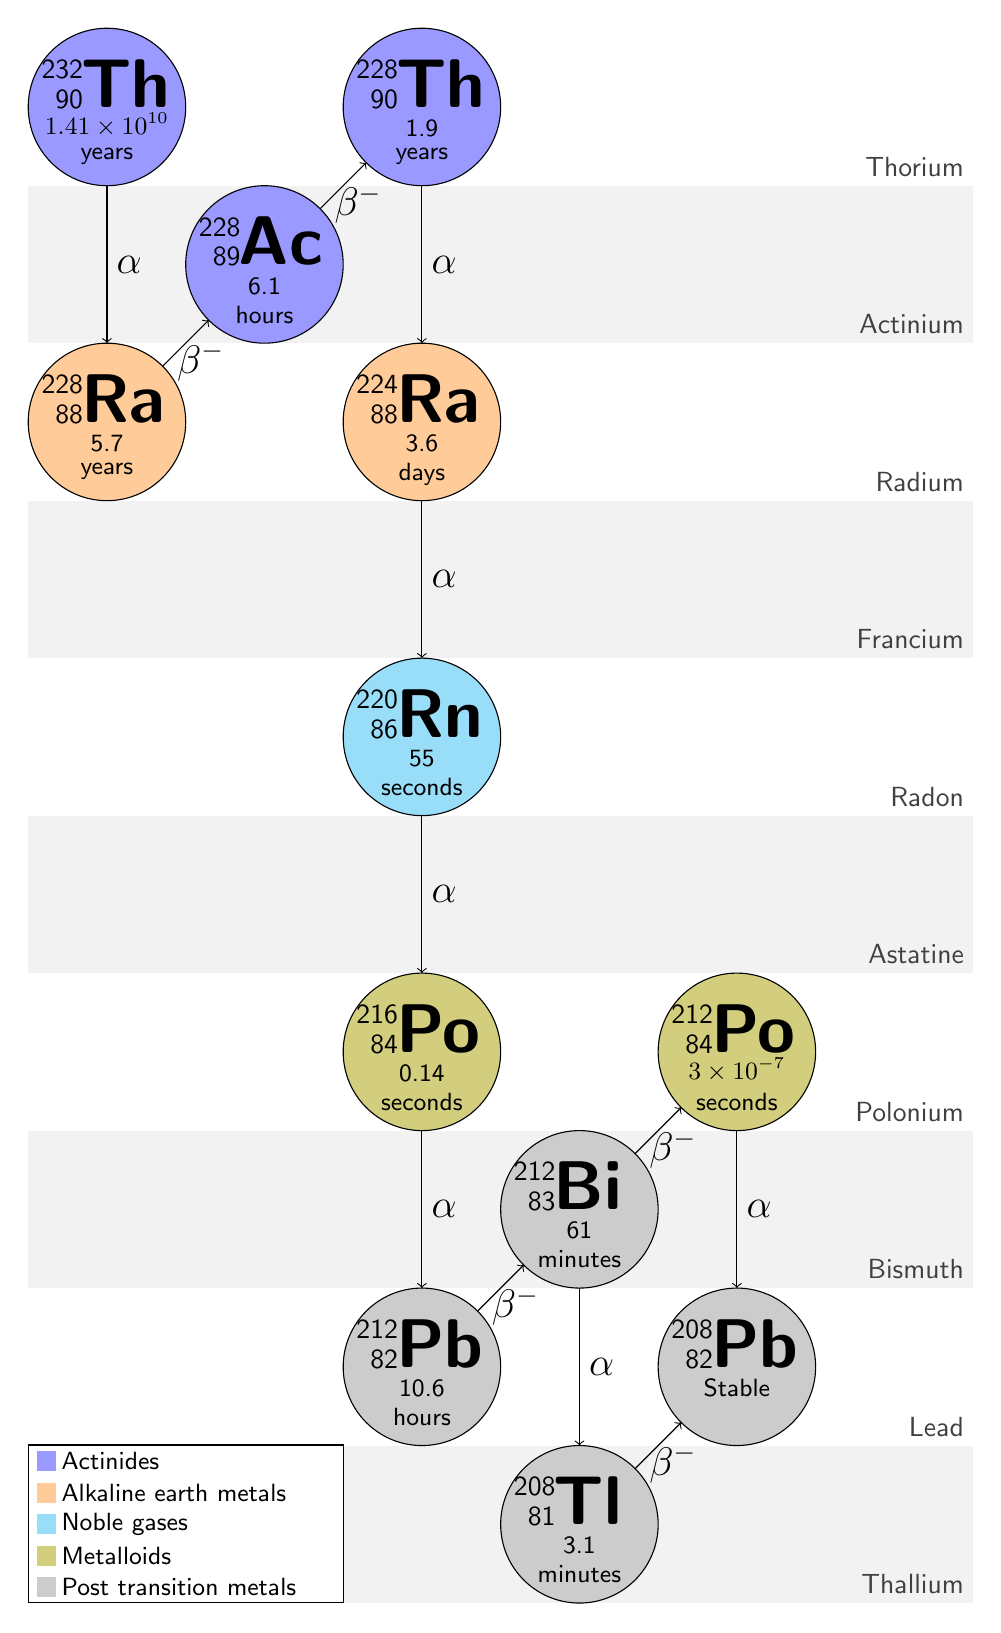
\begin{tikzpicture}
  \sffamily
  \def\nucleus#1#2#3#4#5#6#7#8{
    \node[circle,draw,fill=#1!40,minimum size = 2cm] (#2) at (#3,#4){}; %minimum size = diameter of the circle.
    \node[anchor=west,font=\Huge] at (#3-0.45,#4+0.3){\textbf{#2}};
    \node[anchor=east,font=\normalsize] at (#3-0.18,#4+0.475){#5};
    \node[anchor=east,font=\normalsize] at (#3-0.18,#4+0.1){#6};
    \node[anchor=south,font=\small] at (#3,#4-0.5){#7};
    \node[anchor=north,font=\small] at (#3,#4-0.4){#8};
  }

  \def\rect#1#2#3#4{
    \node[rectangle,
      %draw = white,
      fill = #3!10,
      minimum width = 12cm,
      minimum height = 2cm] (r) at (#1,#2) {};
    \node[anchor=south east,darkgray] at (r.south east) {#4};
  }
  \def\legendd#1#2#3#4{
    \node[rectangle,anchor=west,thin,fill=#3!40,minimum width = 0.25cm,minimum height = 0.25cm] at (#1,#2){};
    \node[anchor=west,font=\small] at (#1+0.2,#2){#4};
  }

  % Gray-white bands
  \rect{5}{0}{white}{Thorium}
  \rect{5}{-2}{gray}{Actinium}
  \rect{5}{-4}{white}{Radium}
  \rect{5}{-6}{gray}{Francium}
  \rect{5}{-8}{white}{Radon}
  \rect{5}{-10}{gray}{Astatine}
  \rect{5}{-12}{white}{Polonium}
  \rect{5}{-14}{gray}{Bismuth}
  \rect{5}{-16}{white}{Lead}
  \rect{5}{-18}{gray}{Thallium}

  % Legend
  \node[rectangle,anchor=south west,thin,draw=black,fill=white,minimum width = 4cm,minimum height = 2cm] at (-1,-19){};
  \legendd{-1+0.1}{-17.2}{blue}{Actinides}
  \legendd{-1+0.1}{-17.6}{orange}{Alkaline earth metals}
  \legendd{-1+0.1}{-18}{cyan}{Noble gases}
  \legendd{-1+0.1}{-18.4}{olive}{Metalloids}
  \legendd{-1+0.1}{-18.8}{gray}{Post transition metals}

  % Nuclei
  \nucleus{blue}{Th}{0}{0}{232}{90}{$1.41\times 10^{10}$}{years}
  \draw[-{>[scale=2]},thin,font=\Large] (0,-1) -- node[right]{$\alpha$} (0,-3);

  \nucleus{orange}{Ra}{0}{-4}{228}{88}{5.7}{years}
  \draw[-{>[scale=2]},thin,font=\Large] (0.707,-3.293) -- node[right,pos=0.1]{$\beta^-$} (1.293,-2.707);

  \nucleus{blue}{Ac}{2}{-2}{228}{89}{6.1}{hours}
  \draw[-{>[scale=2]},thin,font=\Large] (2.707,-1.293) -- node[right,pos=0.1]{$\beta^-$} (3.293,-0.707);

  \nucleus{blue}{Th}{4}{0}{228}{90}{1.9}{years}
  \draw[-{>[scale=2]},thin,font=\Large] (4,-1) -- node[right]{$\alpha$} (4,-3);

  \nucleus{orange}{Ra}{4}{-4}{224}{88}{3.6}{days}
  \draw[-{>[scale=2]},thin,font=\Large] (4,-5) -- node[right]{$\alpha$} (4,-7);

  \nucleus{cyan}{Rn}{4}{-8}{220}{86}{55}{seconds}
  \draw[-{>[scale=2]},thin,font=\Large] (4,-9) -- node[right]{$\alpha$} (4,-11);

  \nucleus{olive}{Po}{4}{-12}{216}{84}{0.14}{seconds}
  \draw[-{>[scale=2]},thin,font=\Large] (4,-13) -- node[right]{$\alpha$} (4,-15);

  \nucleus{gray}{Pb}{4}{-16}{212}{82}{10.6}{hours}
  \draw[-{>[scale=2]},thin,font=\Large] (4.707,-15.293) -- node[right,pos=0.1]{$\beta^-$} (5.293,-14.707);

  \nucleus{gray}{Bi}{6}{-14}{212}{83}{61}{minutes}
  \draw[-{>[scale=2]},thin,font=\Large] (6.707,-13.293) -- node[right,pos=0.1]{$\beta^-$} (7.293,-12.707);

  \nucleus{olive}{Po}{8}{-12}{212}{84}{$3\times10^{-7}$}{seconds}
  \draw[-{>[scale=2]},thin,font=\Large] (6,-15) -- node[right]{$\alpha$} (6,-17);

  \nucleus{gray}{Pb}{8}{-16}{208}{82}{Stable}{}
  \draw[-{>[scale=2]},thin,font=\Large] (8,-13) -- node[right]{$\alpha$} (8,-15);

  \nucleus{gray}{Tl}{6}{-18}{208}{81}{3.1}{minutes}
  \draw[-{>[scale=2]},thin,font=\Large] (6.707,-17.293) -- node[right,pos=0.1]{$\beta^-$} (7.293,-16.707);

\end{tikzpicture}
\end{document}